\documentclass[sigconf]{acmart}
\usepackage[pdf]{graphviz}
\begin{document}

\title{Pennant Lines: An Alternative to Finger Trees in Dynamic Environments}

\author{Daniel Jay Haskin}
\email{dan@djhaskin.com}
\renewcommand{\shortauthors}{Haskin}

\begin{abstract}
Pennant Lines are presented, a novel data structure for storing persistent
sequences in Common Lisp suitable as a drop-in replacement for normal lists, but
with much better runtimes for most operations. These sequences support at least
logarithmic time when implementing a version of the Common Lisp Sequences API
persistently, and better time in other key cases. All are simpler to implement
within a dynamic setting such as that of Common Lisp than Finger Trees, and play
nicer with the larger Lisp ecosystem.
\end{abstract}

%% https://dl.acm.org/ccs.cfm
\begin{CCSXML}
<ccs2012>
<concept>
<concept_id>10003752.10003809.10010031</concept_id>
<concept_desc>Theory of computation~Data structures design and analysis</concept_desc>
<concept_significance>500</concept_significance>
</concept>
</ccs2012>
\end{CCSXML}
\ccsdesc[500]{Theory of computation~Data structures design and analysis}
\keywords{lisp, datastructure, sequences, dynamic, untyped}

%%\begin{teaserfigure}
%%  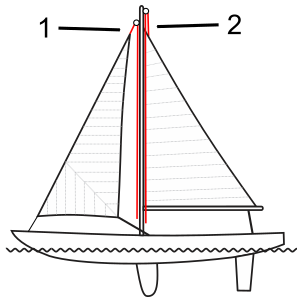
\includegraphics[width=\textwidth]{img/Halyard}
%%  \caption{A depiction of a Halyard[1].}
%%  \Description{A drawing of a sailbosat with the main and jib halyards
%%    highlighted.}
%%  \label{fig:teaser}
%%\end{teaserfigure}

%%\received{20 February 2007}
%%\received[revised]{12 March 2009}
%%\received[accepted]{5 June 2009}
\maketitle

\section{Motivation}

When in a dynamically typed language like Lisp, it is often convenient to work
with a data structure in specific ways in one moment, such as for operating on
sets, and then perform simple list operations on them the next. Alists are nice
because at the end of the day, "they are just lists" -- they can be fed into
functions that expect an array of items, like \texttt{print}. Object type is fluid in
Lisp, as is object purpose. In Lisp, data structures can be used for their
characteristics and ergonomics, rather than for their intended type. Lisp is
a highly dynamic environment.

In the dynamic environment of Common Lisp, lists are used for  \emph{everything}, from
dictionaries to sets to arrays. All the tooling works better with these data
structures than with anything else. Getting the nth element, performing set
union or intersection, stack operations, and syntax abstractions on lists are
all defined in the Common Lisp standard.

However, lists present poor run time characteristics when used for anything more
complicated than a stack. Often lists are used simply because of their ease of
use with little regard for runtime. This is fine until the runtime becomes
important; then ergonomics is sacrificed and the code is rewritten data
structures which are faster, but less ergonomic.

We wish to implement the Common Lisp list and sequence API in a way which is
ergonomic, persistent by default, and dynamic. This means the resulting data
structure must be usable as a list first, but sometimes also as a set or
dictionary. By implementing the list API, we make it easy for people to use the
structure, since all the functions they are used to using with lists exist and
work just as they do for lists, they just exist in a different package.

As a first attempt at this task, Finger Trees\cite{Hinze-Paterson:FingerTree}
were first examined. The problem with Finger Trees is that, while they are easy
to implement in Haskell, with its algebraic sum types and pattern matching, they
are clunky to implement in a dynamically typed language like Lisp. Implementing
Finger Trees involves polymorphic recursion. Every level in a finger tree
contains deeper 2-3 trees than the level above it, and values are only at the
leaves. The spine of the tree is different than the leaves.

This creates a lot of case-by-case work in Lisp. The CLOS is well designed, but
can be slow, especially in the "hot path" in which data structure operations
often find themselves. Without using the CLOS, we are left with the choice of
using \texttt{defstruct} and \texttt{typecase}, which greatly complicates the implementation.
This is especially true in a language without built-in support for pattern
matching like Lisp.

It would be ideal if the data structure were relatively homogeneous -- it looked
the same throughout. This would greatly decrease case logic.
%% We also want structure that is cons-based. That way, it is still "just a list"
%% and can work with a lot of list tooling --
%$% \texttt{destructuring-bind}, \texttt{copy-tree}, \texttt{tree-equal},
%% \texttt{print}, etc.

Finally, we need a structure that is tolerant to and implements functionality
for non-persistent updates along side the persistent ones. This mirrors how
lists are used in Common Lisp -- persistent by default, but changeable if need
be.

So, we need to create a data structure that is relatively homogeneous, with
few cases to manage. It must be able to be used dynamically for different
purposes. It must be persistent by default, but changeable if needed. Most
important, it should have good running time when implementing the Common Lisp
Standard's List API is implemented.

\section{Development}

In this section we first lay out the API that needs to be implemented and summarize
what functionality needs to exist for that API. We then develop an answer to
that API with weight-balanced binary trees. Finally, develop even better run
times by adding pennant lines to the mix.

Here is the API for lists which we will implement, or in some cases, reuse:

\begin{itemize}
    \item \texttt{subst}, \texttt{subst-if}, \texttt{subst-if-not}
    \item \texttt{sublis}
    \item \texttt{atom}
    \item \texttt{copy-tree}
    \item \texttt{tree-equal}
    \item \texttt{copy-list}
    \item \texttt{list-length}
    \item \texttt{list}, \texttt{list*}, \texttt{make-list}
    \item \texttt{listp}
    \item \texttt{push}
    \item \texttt{pop}
    \item \texttt{nth}
    \item \texttt{null}
    \item \texttt{butlast}
    \item \texttt{pairlis}
    \item \texttt{assoc}
    \item \texttt{subsetp}
    \item \texttt{union}
    \item \texttt{intersection}
    \item \texttt{set-difference}
    \item \texttt{set-exclusive-or}
    \item \texttt{pushnew}
    \item \texttt{first}..\texttt{tenth}
    \item \texttt{cons}
    \item \texttt{acons}
    \item \texttt{endp}
    \item \texttt{ldiff}
    \item \texttt{tailp}
    \item \texttt{rest}
    \item \texttt{member}, \texttt{member-if}, \texttt{member-if-not}
    \item \texttt{map*} functions
\end{itemize}

Also mutating versions:

\begin{itemize}
    \item \texttt{rplaca}, \texttt{rplacd}
    \item \texttt{nconc}
    \item \texttt{nsubst}, \texttt{nsubst-if}, \texttt{nsubst-if-not}
    \item \texttt{nbutlast}
\end{itemize}

We also must deal with the generic sequences API. Here are the functions we
choose to implement from that API:

Functions that modify the original structure:


\begin{itemize}
    \item \texttt{delete}, \texttt{delete-if}, \texttt{delete-if-not}
    \item \texttt{nsubstitute-if}, \texttt{nsubstitute-if-not}
    \item \texttt{fill}
    \item \texttt{map-into}
    \item \texttt{replace}
    \item \texttt{nsubstitute}
\end{itemize}

Functions that don't care what the sequence is, they just need one (and
therefore traversal needs to be kinda fast, hopefully somewhat
locality-respecting).

\begin{itemize}
    \item \texttt{map}
    \item \texttt{reduce}
    \item \texttt{count-if}, \texttt{count-if-noT}
    \item \texttt{find-if}, \texttt{find-if-not}
    \item \texttt{position-if}, \texttt{position-if-not}
    \item \texttt{substitute-if}, \texttt{substitute-if-not}
    \item \texttt{remove-if}, \texttt{remove-if-not},
    \item \texttt{search}
    \item \texttt{sort}, \texttt{stable-sort} (sets sorted flag)
\end{itemize}

Functions that can be implemented persistently and therefore need to be "kinda
fast":

\begin{itemize}
    \item \texttt{elt}
    \item \texttt{copy-seq}
    \item \texttt{make-sequence}
    \item \texttt{subseq}
    \item \texttt{count}
    \item \texttt{length}
    \item \texttt{reverse}
    \item \texttt{find} (check if sorted, check the sorted flag)
    \item \texttt{position} (check if sorted)
    \item \texttt{mismatch} (check if sorted)
    \item \texttt{substitute} (
    \item \texttt{concatenate}
    \item \texttt{merge}
    \item \texttt{remove}
    \item \texttt{remove-duplicates} (tree's left arm is \texttt{<=}, multiset)
\end{itemize}

(We will likely have to pare this down a bit, but it's still an interesting
idea)

These APIs boils down to a persistent-by-default structure supporting the following:

\begin{itemize}
    \item Efficient random insertion, deletion, and access (IDA)
    \item Efficient IDA at the ends
    \item Efficient traversal
    \item Efficient concatenation
    \item Efficient splitting
    \item Efficient set operations
\end{itemize}

It would also be nice to reuse some of the functions, like \texttt{tree-equal} and
\texttt{copy-tree}.


\section{Tables}


Immediately following this sentence is the point at which
Table~\ref{tab:freq} is included in the input file; compare the
placement of the table here with the table in the printed output of
this document.

\begin{table}
  \caption{Frequency of Special Characters}
  \label{tab:freq}
  \begin{tabular}{ccl}
    \toprule
    Non-English or Math&Frequency&Comments\\
    \midrule
    \O & 1 in 1,000& For Swedish names\\
    $\pi$ & 1 in 5& Common in math\\
    \$ & 4 in 5 & Used in business\\
    $\Psi^2_1$ & 1 in 40,000& Unexplained usage\\
  \bottomrule
\end{tabular}
\end{table}

To set a wider table, which takes up the whole width of the page's
live area, use the environment \textbf{table*} to enclose the table's
contents and the table caption.  As with a single-column table, this
wide table will \texttt{''float} to a location deemed more
desirable. Immediately following this sentence is the point at which
Table~\ref{tab:commands} is included in the input file; again, it is
instructive to compare the placement of the table here with the table
in the printed output of this document.

\begin{table*}
  \caption{Some Typical Commands}
  \label{tab:commands}
  \begin{tabular}{ccl}
    \toprule
    Command &A Number & Comments\\
    \midrule
    \texttt{{\char'134}author} & 100& Author \\
    \texttt{{\char'134}table}& 300 & For tables\\
    \texttt{{\char'134}table*}& 400& For wider tables\\
    \bottomrule
  \end{tabular}
\end{table*}

Always use midrule to separate table header rows from data rows, and
use it only for this purpose. This enables assistive technologies to
recognise table headers and support their users in navigating tables
more easily.

\section{Math Equations}
You may want to display math equations in three distinct styles:
inline, numbered or non-numbered display.  Each of the three are
discussed in the next sections.

\subsection{Inline (In-text) Equations}
A formula that appears in the running text is called an inline or
in-text formula.  It is produced by the \textbf{math} environment,
which can be invoked with the usual
\texttt{{\char'134}begin\,\ldots{\char'134}end} construction or with
the short form \texttt{\$\,\ldots\$}. You can use any of the symbols
and structures, from $\alpha$ to $\omega$, available in
\LaTeX~\cite{Lamport:LaTeX}; this section will simply show a few
examples of in-text equations in context. Notice how this equation:
\begin{math}
  \lim_{n\rightarrow \infty}x=0
\end{math},
set here in in-line math style, looks slightly different when
set in display style.  (See next section).

\subsection{Display Equations}
A numbered display equation---one set off by vertical space from the
text and centered horizontally---is produced by the \textbf{equation}
environment. An unnumbered display equation is produced by the
\textbf{displaymath} environment.

Again, in either environment, you can use any of the symbols and
structures available in \LaTeX\@; this section will just give a couple
of examples of display equations in context.  First, consider the
equation, shown as an inline equation above:
\begin{equation}
  \lim_{n\rightarrow \infty}x=0
\end{equation}
Notice how it is formatted somewhat differently in
the \textbf{displaymath}
environment.  Now, we'll enter an unnumbered equation:
\begin{displaymath}
  \sum_{i=0}^{\infty} x + 1
\end{displaymath}
and follow it with another numbered equation:
\begin{equation}
  \sum_{i=0}^{\infty}x_i=\int_{0}^{\pi+2} f
\end{equation}
just to demonstrate \LaTeX's able handling of numbering.

\section{Figures}

\begin{figure}[h]
  \centering
  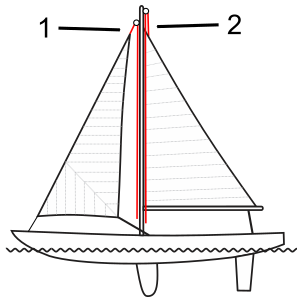
\includegraphics[width=\linewidth]{img/Halyard}
  \caption{1907 Franklin Model D roadster. Photograph by Harris \&
    Ewing, Inc. [Public domain], via Wikimedia
    Commons. (\url{https://goo.gl/VLCRBB}).}
  \Description{A woman and a girl in white dresses sit in an open car.}
\end{figure}

so important, please see
\url{https://www.acm.org/publications/taps/describing-figures/}.

\section{Citations and Bibliographies}

\begin{acks}
    Thanks is due to Dr. Kimball Germane of Brigham Young University, Provo,
    Utah for previewing drafts and offering feedback.
\end{acks}

%%
%% The next two lines define the bibliography style to be used, and
%% the bibliography file.
\bibliographystyle{ACM-Reference-Format}
\bibliography{pennant-lines}

%%
%% If your work has an appendix, this is the place to put it.
\appendix

\section{Research Methods}

\subsection{Part One}

Lorem ipsum dolor sit amet, consectetur adipiscing elit. Morbi
malesuada, quam in pulvinar varius, metus nunc fermentum urna, id
sollicitudin purus odio sit amet enim. Aliquam ullamcorper eu ipsum
vel mollis. Curabitur quis dictum nisl. Phasellus vel semper risus, et
lacinia dolor. Integer ultricies commodo sem nec semper.

\subsection{Part Two}

Etiam commodo feugiat nisl pulvinar pellentesque. Etiam auctor sodales
ligula, non varius nibh pulvinar semper. Suspendisse nec lectus non
ipsum convallis congue hendrerit vitae sapien. Donec at laoreet
eros. Vivamus non purus placerat, scelerisque diam eu, cursus
ante. Etiam aliquam tortor auctor efficitur mattis.

\section{Online Resources}

Nam id fermentum dui. Suspendisse sagittis tortor a nulla mollis, in
pulvinar ex pretium. Sed interdum orci quis metus euismod, et sagittis
enim maximus. Vestibulum gravida massa ut felis suscipit
congue. Quisque mattis elit a risus ultrices commodo venenatis eget
dui. Etiam sagittis eleifend elementum.

Nam interdum magna at lectus dignissim, ac dignissim lorem
rhoncus. Maecenas eu arcu ac neque placerat aliquam. Nunc pulvinar
massa et mattis lacinia.

\end{document}
\endinput
%%
%% End of file `sample-sigconf-authordraft.tex'.
